\section{Communication protocols}
\label{sec:comm_protocols}
According to the thesis instruction and the requirements \textbf{FR-04}, \textbf{NFR-02}, \textbf{C-03}, \textbf{C-05},  the stepper driver should feature CANOpen and I2C interfaces for control and configuration and the USB interface for configuration.
This section aims to give a brief overview into these communication interfaces and protocols utilized with them.

\subsection{CANOpen}
\label{subsec:canopen}



% TODO cite
\subsubsection{CAN bus}
The Controlled Area Network is a bus most commonly used in automotive for connecting ECUs (Electronic Control Units) together.
The bus was developed by Bosch and codified into the ISO11898-1 standard\cite{}.
CAN bus utilizes a single differential pair making simplifying the wiring of a complex system consisting of many ECUs.

On the physical layer, the bus has two states - recessive and dominant, where recessive means that the differential voltage between the CANH and CANL signals is less than a minimum threshold voltage, whereas dominant state means that the differential voltage is higher than the minimal threshold voltage.
The dominant state is achieved by sending a logical 0 through the network, while the recessive state is achieved by sending logical 1.
CAN bus utilizes the CSMA/CD media access control protocol, which allows for collision detection and potential retransmission of CAN frames.
For collision detection, it is vital, that the dominant state overrides a recessive one.

There are two types of frames transmitted on the bus - standard frames and extended frames.
These frames differ in the identifier length, where the extended frame allows for 29 bit long identifier in contrast to the standard frame, that allows for only 11 bits.
Identifier length is selected on per-frame basis using the IDE bit in the frame.
Each CAN frame may contain up to 8 bytes of data and the data length is controlled by the four DLC bits in the frame.
The structure of a CAN frame can be seen in the Figure~\ref{fig:can_frame}.

\begin{figure}[H]
    \centering
    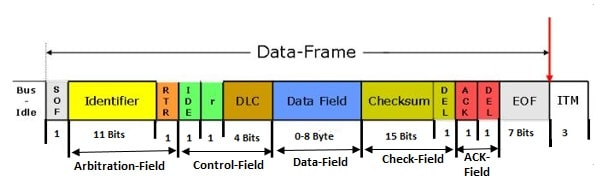
\includegraphics[width=\textwidth]{obrazky/can_frame}
    \caption{CAN bus frame with standard identifier~\cite{piembsystech}.}
    \label{fig:can_frame}
\end{figure}

An important bit for CANOpen is the RTR bit, which stands for Remote Transmission Request, when this bit is recessive, there are no data contained in the frame and the frame asks the remote device for data.
As can be seen in the figure, the identifier and the RTR field are part of an Arbitration field, these bytes are used in the shared medium collision detection and control and thanks to this field, frames with lower id have higher priority in the transmission.

\subsection{I2C}
\label{subsec:i2c}

\subsection{Universal Serial Bus}
\label{subsec:usb}
